\section{放射線試験(寺田(報告書)・池谷・黒崎)}

\subsection{目的}
本試験では,多量の放射線が入射することに起因する電離効果のうち,トータルイオンドーズ効果が機器に与える恒久的損傷を調べた.これにより,新規開発基盤である通信\&インヒビット(CI)基板および膜上デバイス制御(MDC)基板に関して,ミッション期間中に受ける損傷具合を試験した.

\subsection{試験概要}
\subsubsection{試験日時}
第1回

2015年10月20日

\vspace{2ex} 
第2回 

2018年5月28日14時から18時(計4時間.準備と撤収時間も含む.$\gamma$線の照射時間は3時間.)

\vspace{3ex} 
\textbf{コメント}
\begin{itemize}
\item 実験室を予約する場合は,照射時間だけでなく,前後の準備撤収時間を考慮し最低1時間は余分に予約する.
\item 第2回試験では1名のみで当日,準備から実験まで行ったが,照射室とPC等を置く場所は離れているので,2名いた方が準備しやすいと思う.
\end{itemize}
	
\subsubsection{試験場所}
東京工業大学 大岡山キャンパス 大岡山北実験棟1 コバルト60照射室

\vspace{3ex} 
\textbf{コメント}
\begin{itemize}
	\item 予約はメールでやり取りを行う.
\end{itemize}

\subsection{第1回放射線試験}
\label{1RadiationTest}

\subsubsection{試験供試体}
CI基板,MDC基板上のIC.供試体一覧を表\ref{table4-1-1}に示す.

\begin{table}[H]
	\centering
	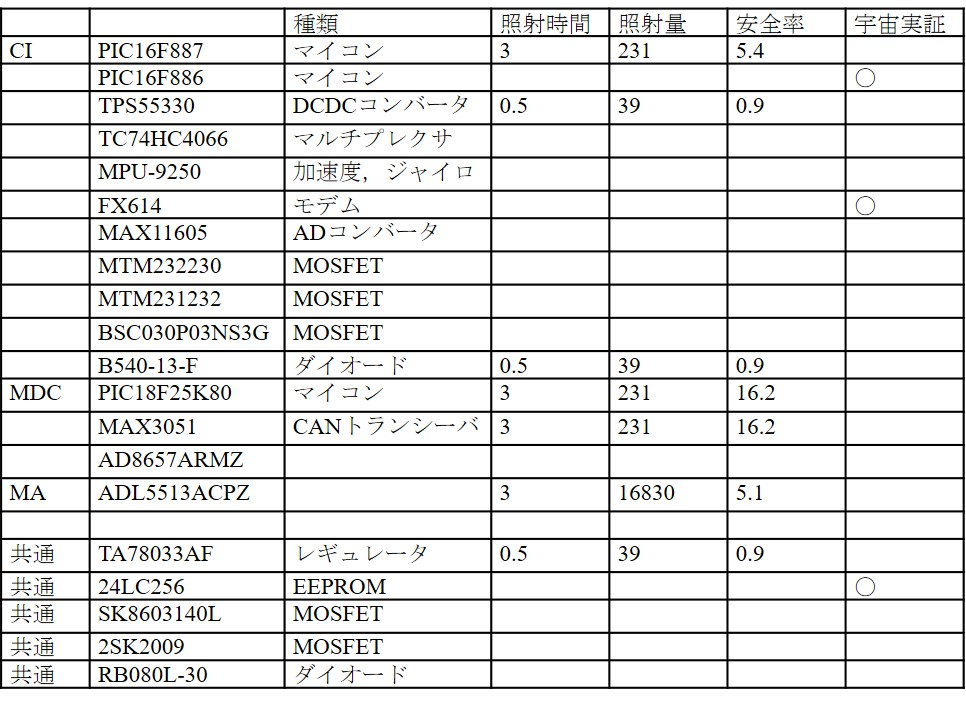
\includegraphics[scale=0.9]{04/fig/t4-1-1.jpg}
	\caption{第1回放射線試験 試験供試体一覧}
	\label{table4-1-1}
\end{table}

\subsubsection{検証方法}
図\ref{fig4-1-0}の通りに,デバイスを配置し,データロガー及びPCでデータをモニタリングした.
\begin{figure}[H]
	\centering
	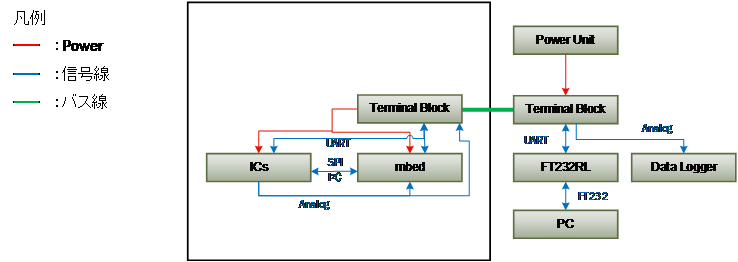
\includegraphics[width=150mm]{04/fig/4-1-0.png}
	\caption{デバイスの位置関係.長方形内が放射線試験室を示している.}
	\label{fig4-1-0}
\end{figure}

\vspace{2ex} 
\textbf{コメント}
\begin{itemize}
	\item 放射線照射室とPC等を置くう照射室外を繋ぐ図\ref{fig4-1-0}の緑ハーネス部分は,コバルト60照射室の設備としてDサブハーネスが既にある.ただ,Dサブハーネスと接続するケーブルは両側,事前に作成しておく必要がある.事前にコバルト60照射室を見学しておくと,どのようなハーネスを作成しなければならないかイメージがつきやすいと思う.
	\item ハーネス作成時には,グラウンドを全て共有することを忘れずに.
\end{itemize}

\subsubsection{照射量}
OrigamiSat-1のCI基板周り,およびMDC基板周りのアルミニウム構体板厚は2 mmである.文献[相互参照使おうね]の厚さ1.85 mm,1年あたりトータルドーズ量4.28E+03 radであるため使用期間をCI基板は1年,MDC基板は4か月として,この値から安全率を計算した.表\ref{table4-1-2}に示す.

11月の線源からの距離60 cmの値74 Gy/hを用いた.
また両基板ともに両面にICが搭載されているため0.5 hごとに基板の表裏をひっくり返した.線源に対して裏面にあるICの被ばく量は表面にあるICの被ばく量に対して微小であると仮定した.

\begin{table}[H]
	\centering
	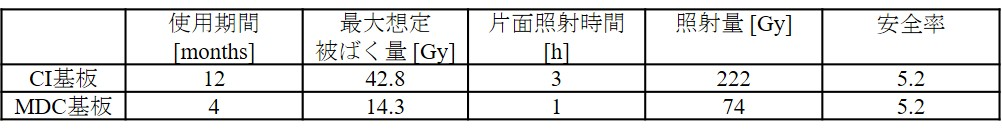
\includegraphics[scale=0.9]{04/fig/t4-1-2.jpg}
	\caption{照射量}
	\label{table4-1-2}
\end{table}


\subsubsection{配置}
線源から60 cm.実験の様子を図\ref{fig4-1-1},図\ref{table4-1-2}に示す.

\begin{figure}[H]
	\centering
	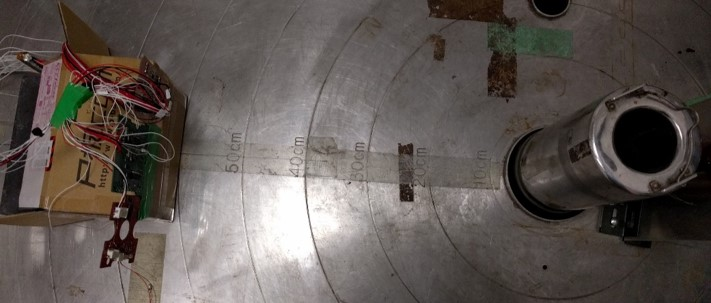
\includegraphics[scale=0.9]{04/fig/4-1-1.jpg}
	\caption{配置の様子}
	\label{fig4-1-1}
\end{figure}
\begin{figure}[H]
	\centering
	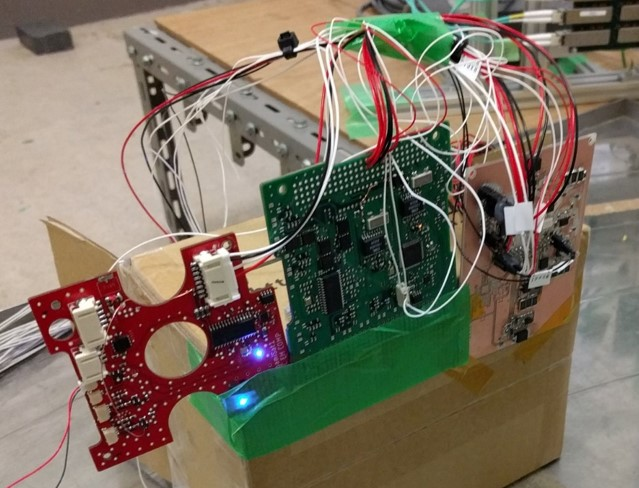
\includegraphics[scale=0.9]{04/fig/4-1-2.jpg}
	\caption{試験供試体拡大図}
\label{fig4-1-2}
\end{figure}

\subsubsection{試験手順}
\begin{itemize}
	\item[ 1. ] 各コンポーネントを接続する
	\item[ 2. ]  順番に電源を投入する
	\item[ 3. ]  照射前に各ICが適切に動作していることを確認する
	\item[ 4. ]  照射:照射中はログを取る
	\item[ 5. ]  撤収する
	\item[ 6. ]  データの解析を行う
\end{itemize}

\vspace{2ex} 
\textbf{コメント}
\begin{itemize}
	\item 試験前日までに,放射線を照射しない状態で予定試験時間分ICが動作することを確認しておく.
\end{itemize}

\subsubsection{試験結果}
\begin{itemize}
	\item[ 結果:] RXCOBCが1.5年分の照射後一時動作不良を引き起こした.
	\item[ 原因:] UARTもしくは$I^{2}C$ラインに不具合が発生したことが原因と思われる.
	\item[ 対策:] PIC16F887をCubeSatでの使用実績のあるPIC16LF877Aに変更.
\end{itemize}

\subsection{第2回放射線試験}
第1回試験でCI基板上のPICにおいて不具合が生じたことを受け,搭載ICの型番を決定するために,3種類のPICにおける追加試験が行われた.また,WDT機能に使用されるSA555タイマーの放射線損傷具合も試験した.

\subsubsection{試験供試体}
CI基板上に搭載されるPICおよびタイマー
\begin{itemize}
	\item PIC:16F886
	\item PIC:16F887
	\item PIC:16LF877A
	\item タイマー:SA555
\end{itemize}

\subsubsection{検証方法}
後で図を追加!!!

\subsubsection{照射量}
\begin{itemize}
	\item 線源からICまでの距離:100cm
	\item 1時間あたりの線量:28.2 Gy/h (参考文献[???]の2017年12月100cmの数値)
	\item 照射時間:3時間
	\item 総照射量:84.6 Gy
\end{itemize}

\vspace{2ex} 
\textbf{コメント}
\begin{itemize}
	\item 第1回試験と行る試験条件(線源までの距離,照射時間)で試験を行ってしまったが,第1回と試験条件を揃えないと,適切に比較はできなかったかもしれない.
\end{itemize}

\subsubsection{配置}
線源から100 cm.

\begin{figure}[H]
	\centering
	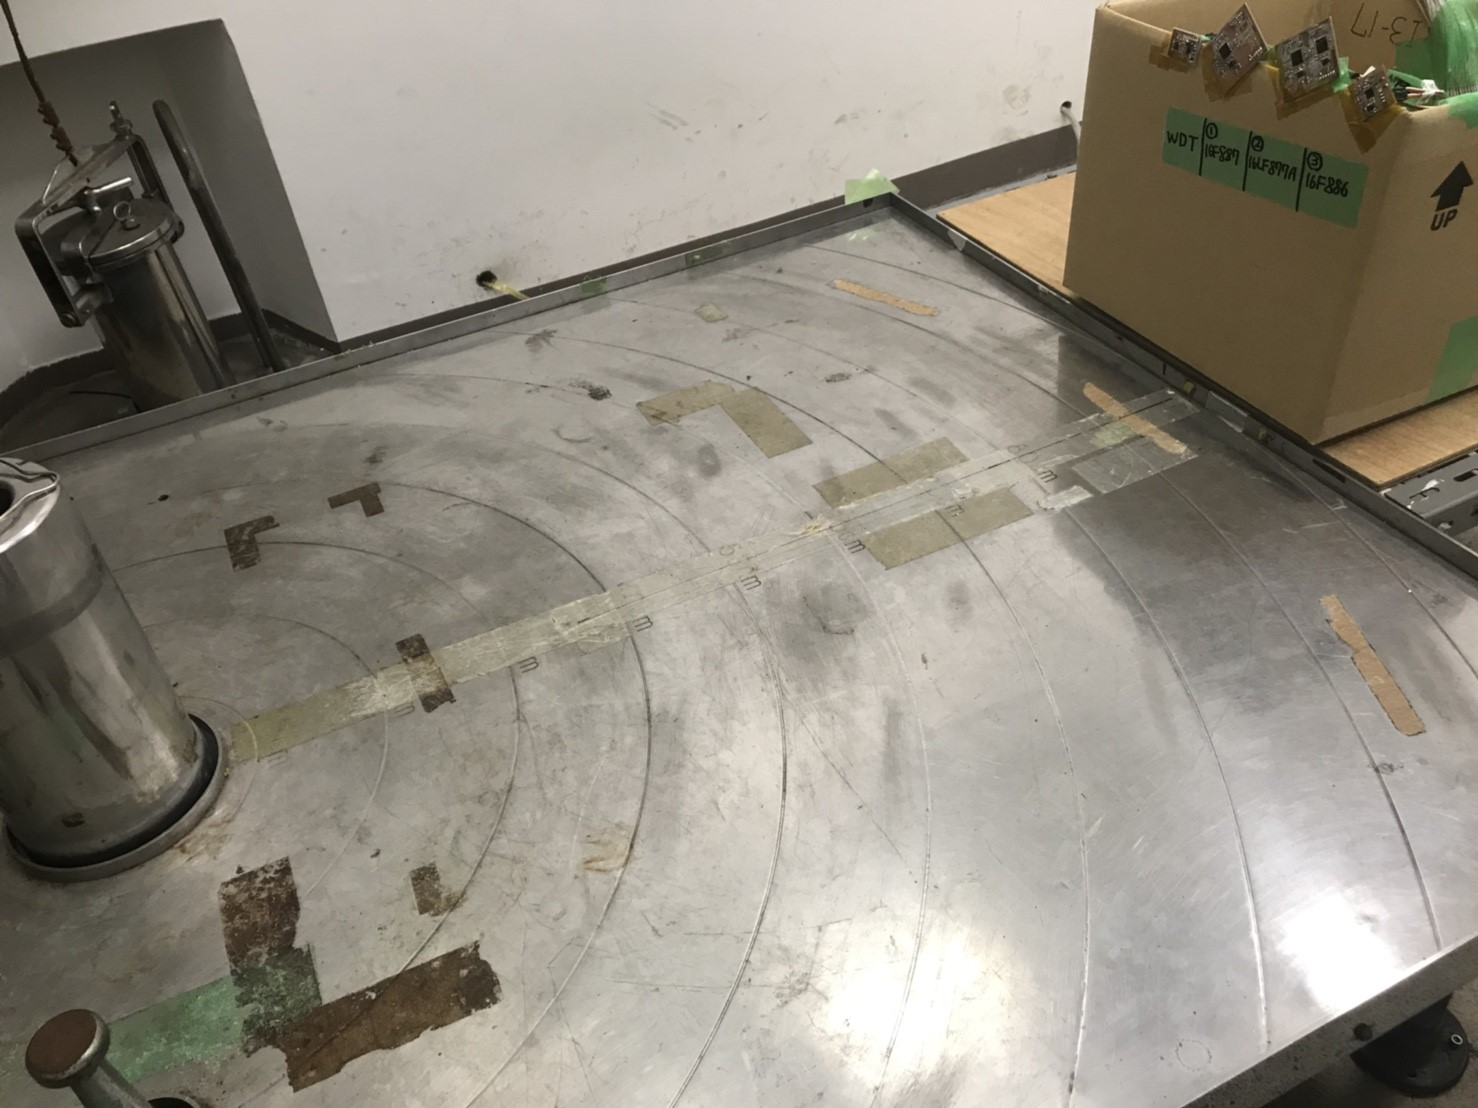
\includegraphics[width=70mm]{04/fig/4-1-3.jpg}
	\caption{配置の様子}
	\label{fig4-1-3}
\end{figure}
\begin{figure}[H]
	\centering
	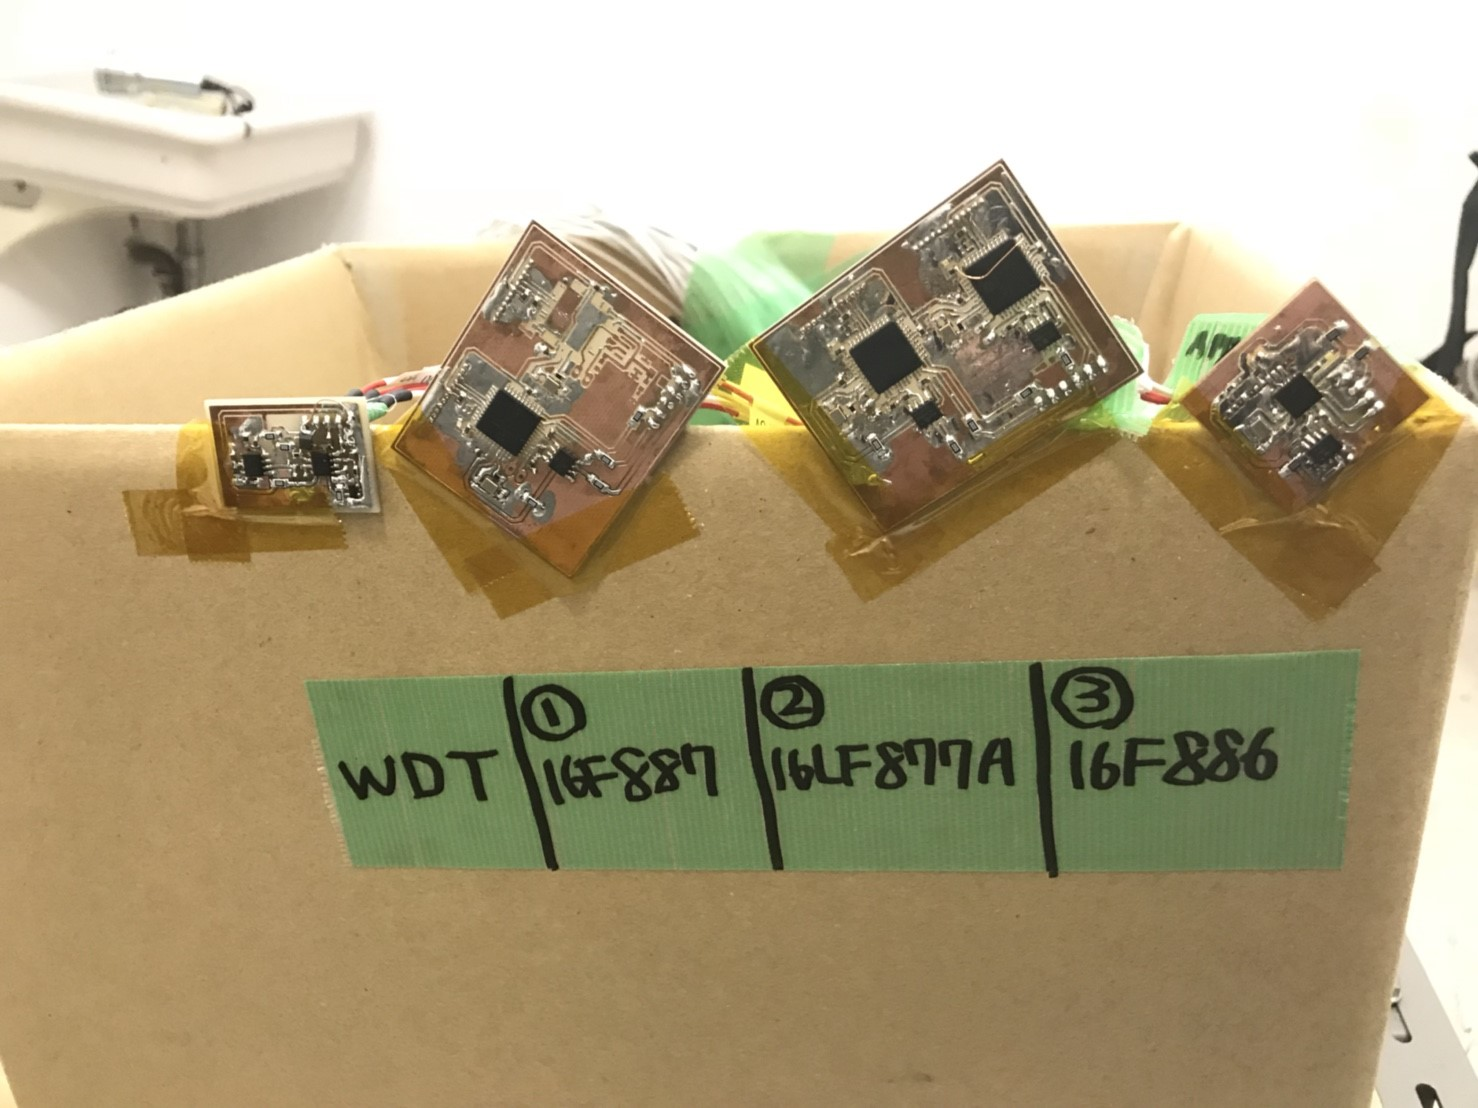
\includegraphics[width=70mm]{04/fig/4-1-4.jpg}
	\caption{試験供試体拡大図}
	\label{fig4-1-4}
\end{figure}
\begin{figure}[H]
	\centering
	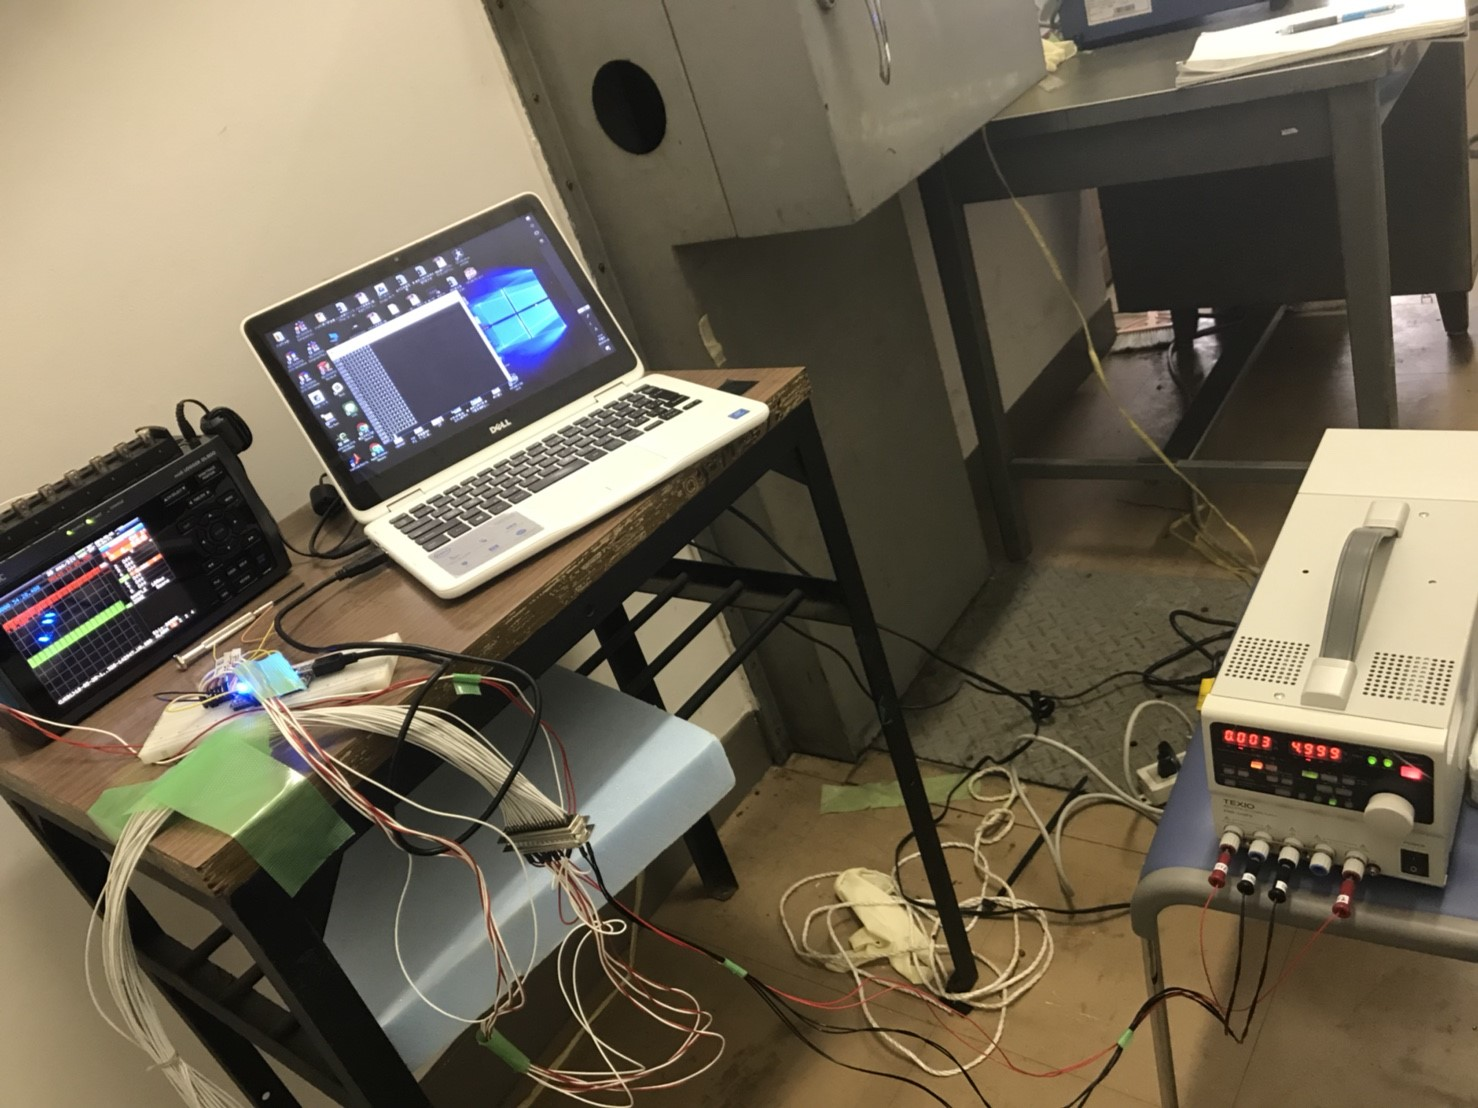
\includegraphics[width=70mm]{04/fig/4-1-5.jpg}
	\caption{照射室外の様子.mbed等が搭載されたブレッドボード,,外部電源,PCなどがある.}
	\label{fig4-1-5}
\end{figure}

\subsubsection{試験手順}
\ref{1RadiationTest}第1回放射線試験(5)試験手順と同様

\subsubsection{試験結果}
\begin{itemize}
	\item[ 結果:]不具合発生せず.RXCOBCは16LF877A,TXCOBCは16F886,タイマーはSA555を採用することに決定.
\end{itemize}
